\chapter{Prototype 2: SyncSpace Architecture Details}
\label{app:syncspace}

This appendix provides a comprehensive technical overview of \textbf{SyncSpace},
the second prototype developed to evaluate the Jakarta EE 11 ecosystem. SyncSpace
is a backend \ac{REST} \ac{API} designed for coworking and meeting-room reservations.
Users authenticate, browse available rooms, and reserve them---either by
selecting a specific room or allowing the system to auto-assign a suitable
one. The application is packaged as a \ac{WAR} and deployed onto a Payara 7
application server, backed by a PostgreSQL database.

\section{Technology Stack}
\label{app:syncspace-stack}

The prototype leverages modern enterprise Java specifications, prioritising standard
APIs over third-party frameworks where possible.

\begin{table}[H]
	\centering
	\renewcommand{\arraystretch}{1.2}
	\begin{tabular}{ll}
		\toprule \textbf{Concern} & \textbf{Technology}                                      \\
		\midrule Platform         & Jakarta EE 11 (\texttt{jakarta.jakartaee-api 11.0.0})    \\
		Profile APIs              & MicroProfile 7.1 (\ac{JWT} auth, Config)                 \\
		App Server                & Payara 7 (embedded for tests)                            \\
		Persistence               & Jakarta Persistence (\ac{JPA}) via EclipseLink           \\
		Data Access               & Jakarta Data repositories (\texttt{CrudRepository})      \\
		Database                  & PostgreSQL (driver 42.7.10)                              \\
		Security                  & MicroProfile \ac{JWT} (RS256 via Nimbus JOSE + \ac{JWT}) \\
		Validation                & Jakarta Bean Validation (Hibernate Validator)            \\
		Test                      & Arquillian + JUnit 5 on embedded Payara                  \\
		Test Data                 & Datafaker 2.5.4                                          \\
		\bottomrule
	\end{tabular}
	\caption{SyncSpace technology stack.}
\end{table}

\section{Architecture and Domain Model}
\label{app:syncspace-arch}

The application follows a clean, layered architecture with strict
separation of concerns. \ac{HTTP} requests enter through \ac{JAX-RS} Resources,
which deserialize and validate payloads before delegating to \texttt{@ApplicationScoped}
Services. These services execute business logic and interact with Jakarta
Data Repositories, which in turn manage \ac{JPA} Entities. Cross-cutting concerns
such as exception mapping and validation surround this core flow.

The domain model relies on three primary entities:
\begin{itemize}
	\item \textbf{User}: Contains credentials and role assignments (\texttt{USER},
		\texttt{ADMIN}).

	\item \textbf{Room}: Defines physical spaces with a specific \texttt{RoomType}
		(e.g., \texttt{HOT\_DESK}, \texttt{BOARDROOM}) and a maximum capacity.

	\item \textbf{Booking}: Links a User and a Room over a specific \texttt{startTime}
		and \texttt{endTime}.
\end{itemize}

\section{Authentication and Security}
\label{app:syncspace-auth}

Security is inherently stateless, relying on asymmetric \ac{JWT} validation.
The \texttt{AuthResource} handles registration and login procedures. During registration,
passwords are hashed using PBKDF2WithHmacSHA256 (10,000 iterations). Upon successful
login, the \texttt{TokenService} issues an RS256-signed \ac{JWT} containing
the user's ID, username, and role claims.

\begin{figure}[H]
	\centering
	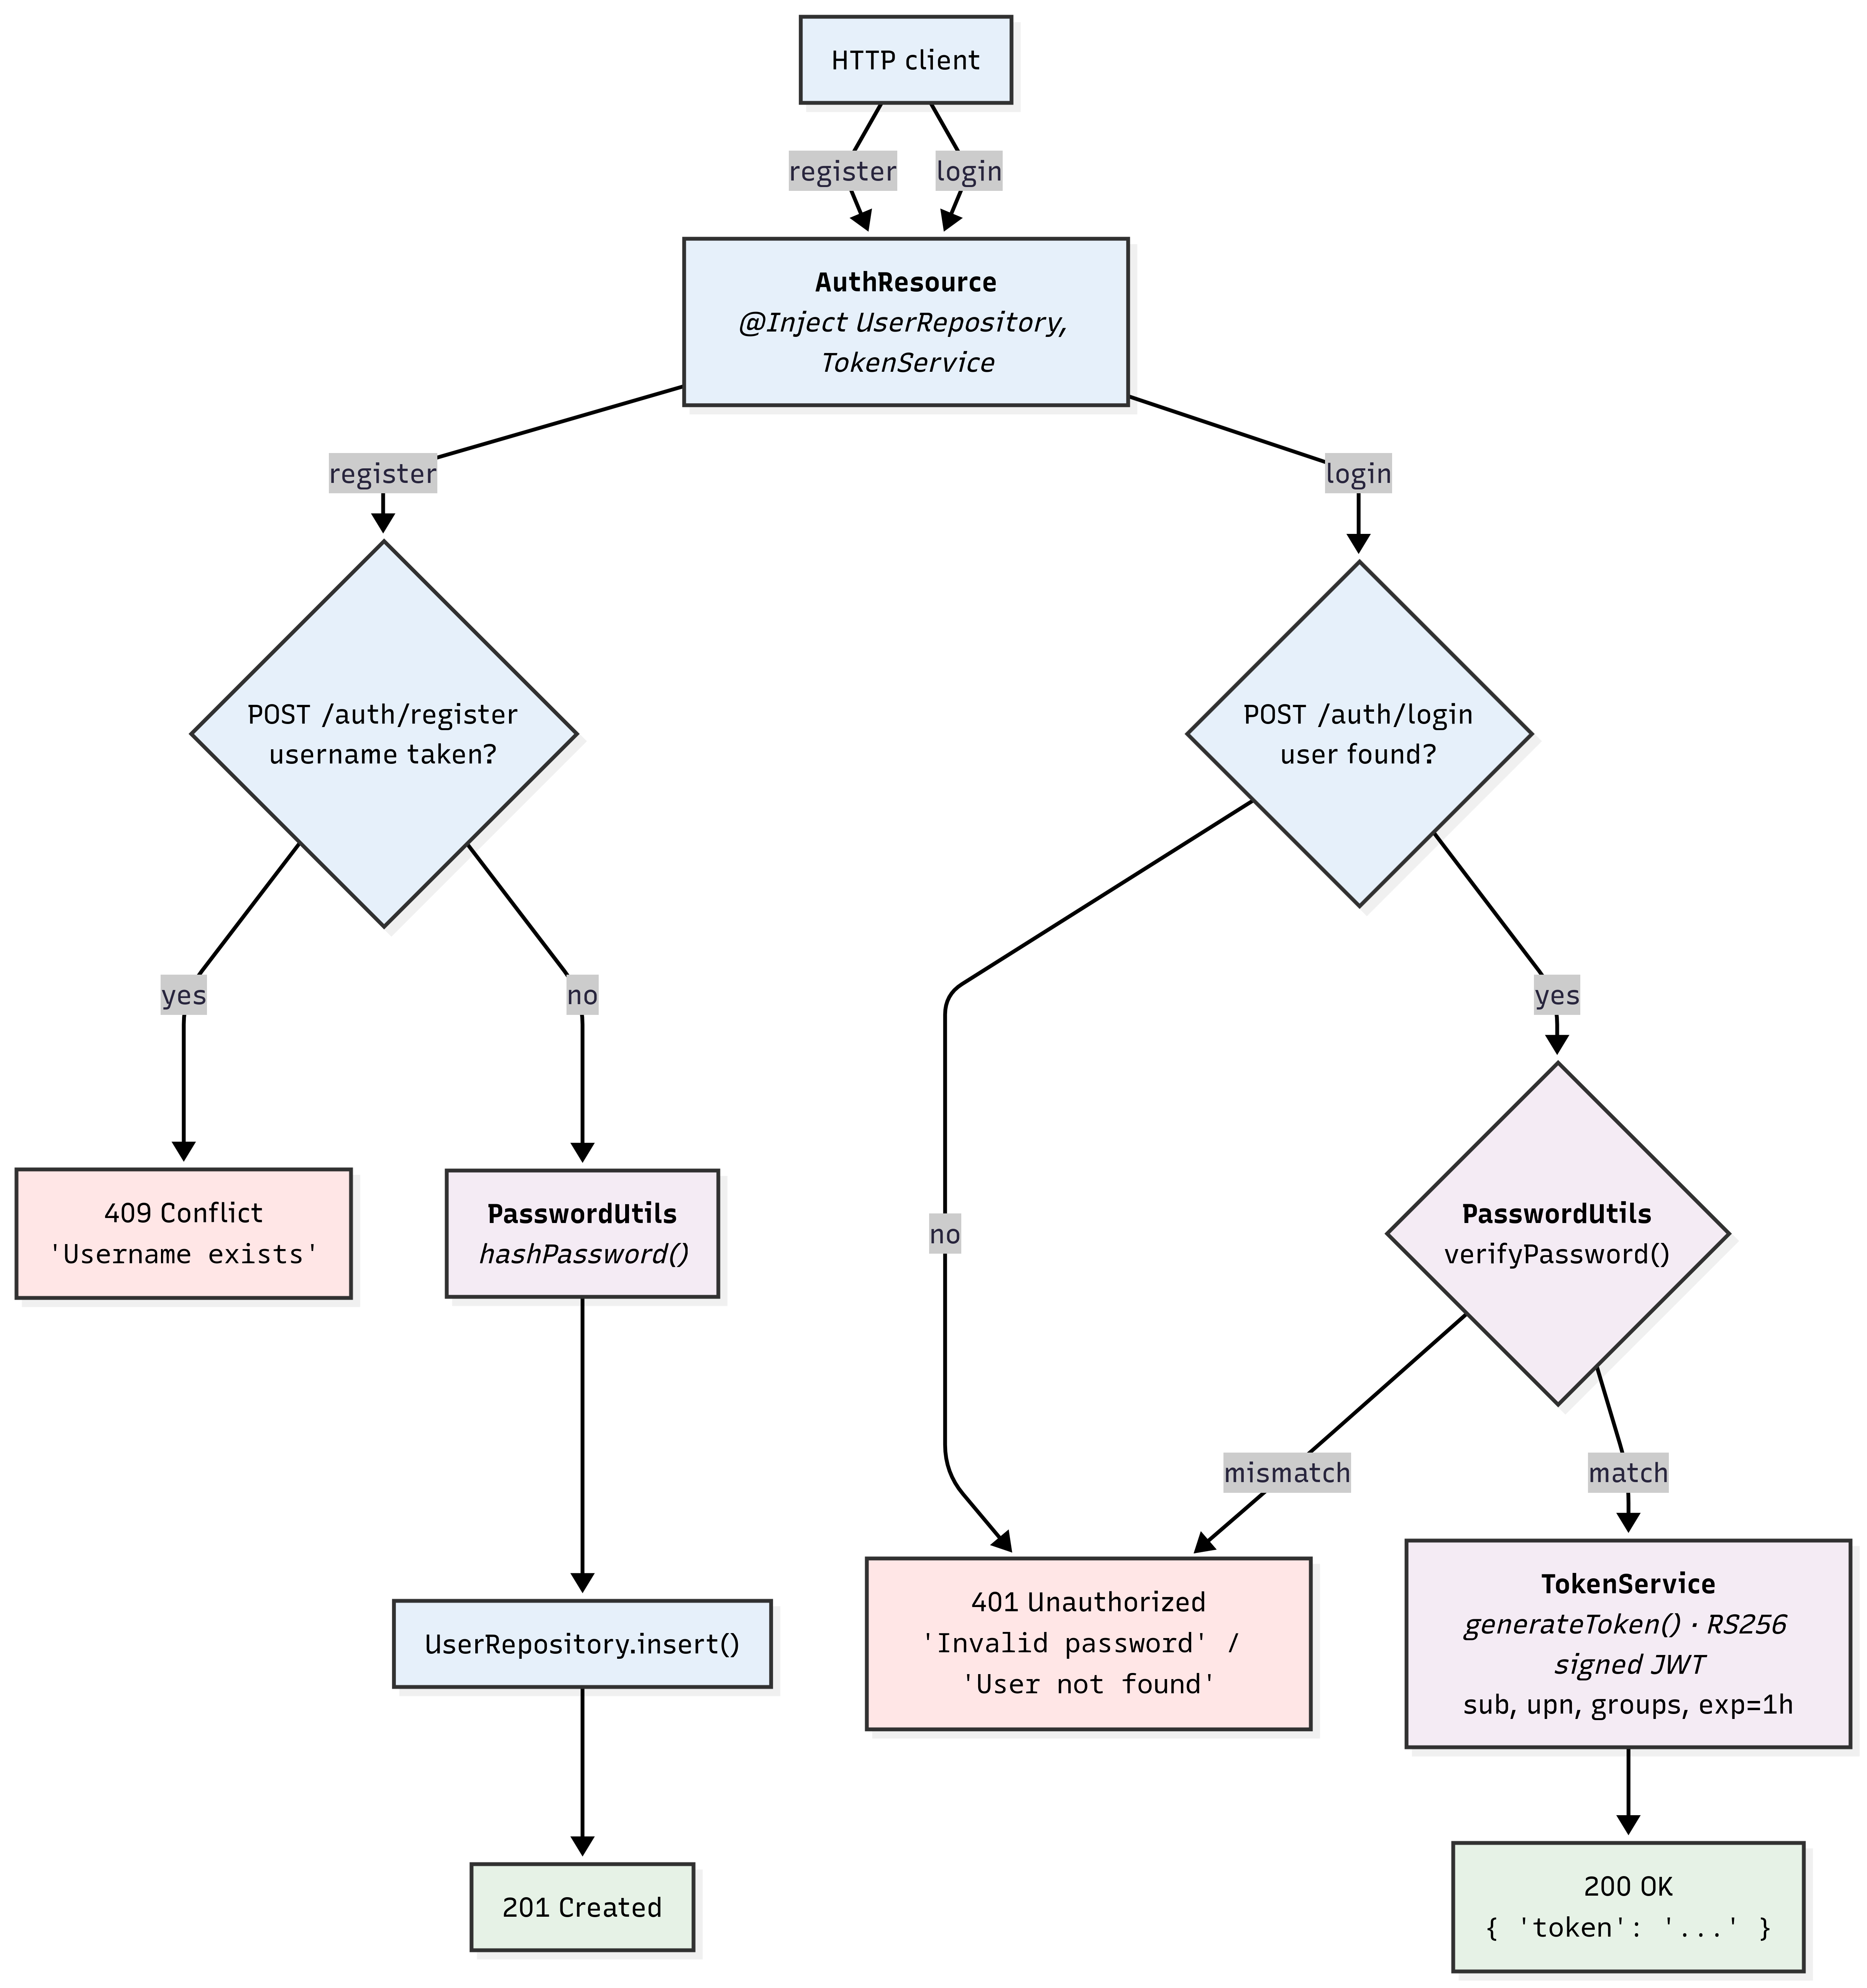
\includegraphics[width=\textwidth, height=10cm, keepaspectratio]{
		diagrams/syncspace-token-issuance.png
	}
	\caption{Token issuance and user registration flow.}
	\label{fig:syncspace-token}
\end{figure}

Incoming requests are intercepted by a MicroProfile \ac{JWT} guard. Payara validates
the signature, issuer, and expiry automatically based on a configured public
key. Role-based authorization is then enforced at the endpoint level via
\texttt{@RolesAllowed} annotations.

\begin{figure}[H]
	\centering
	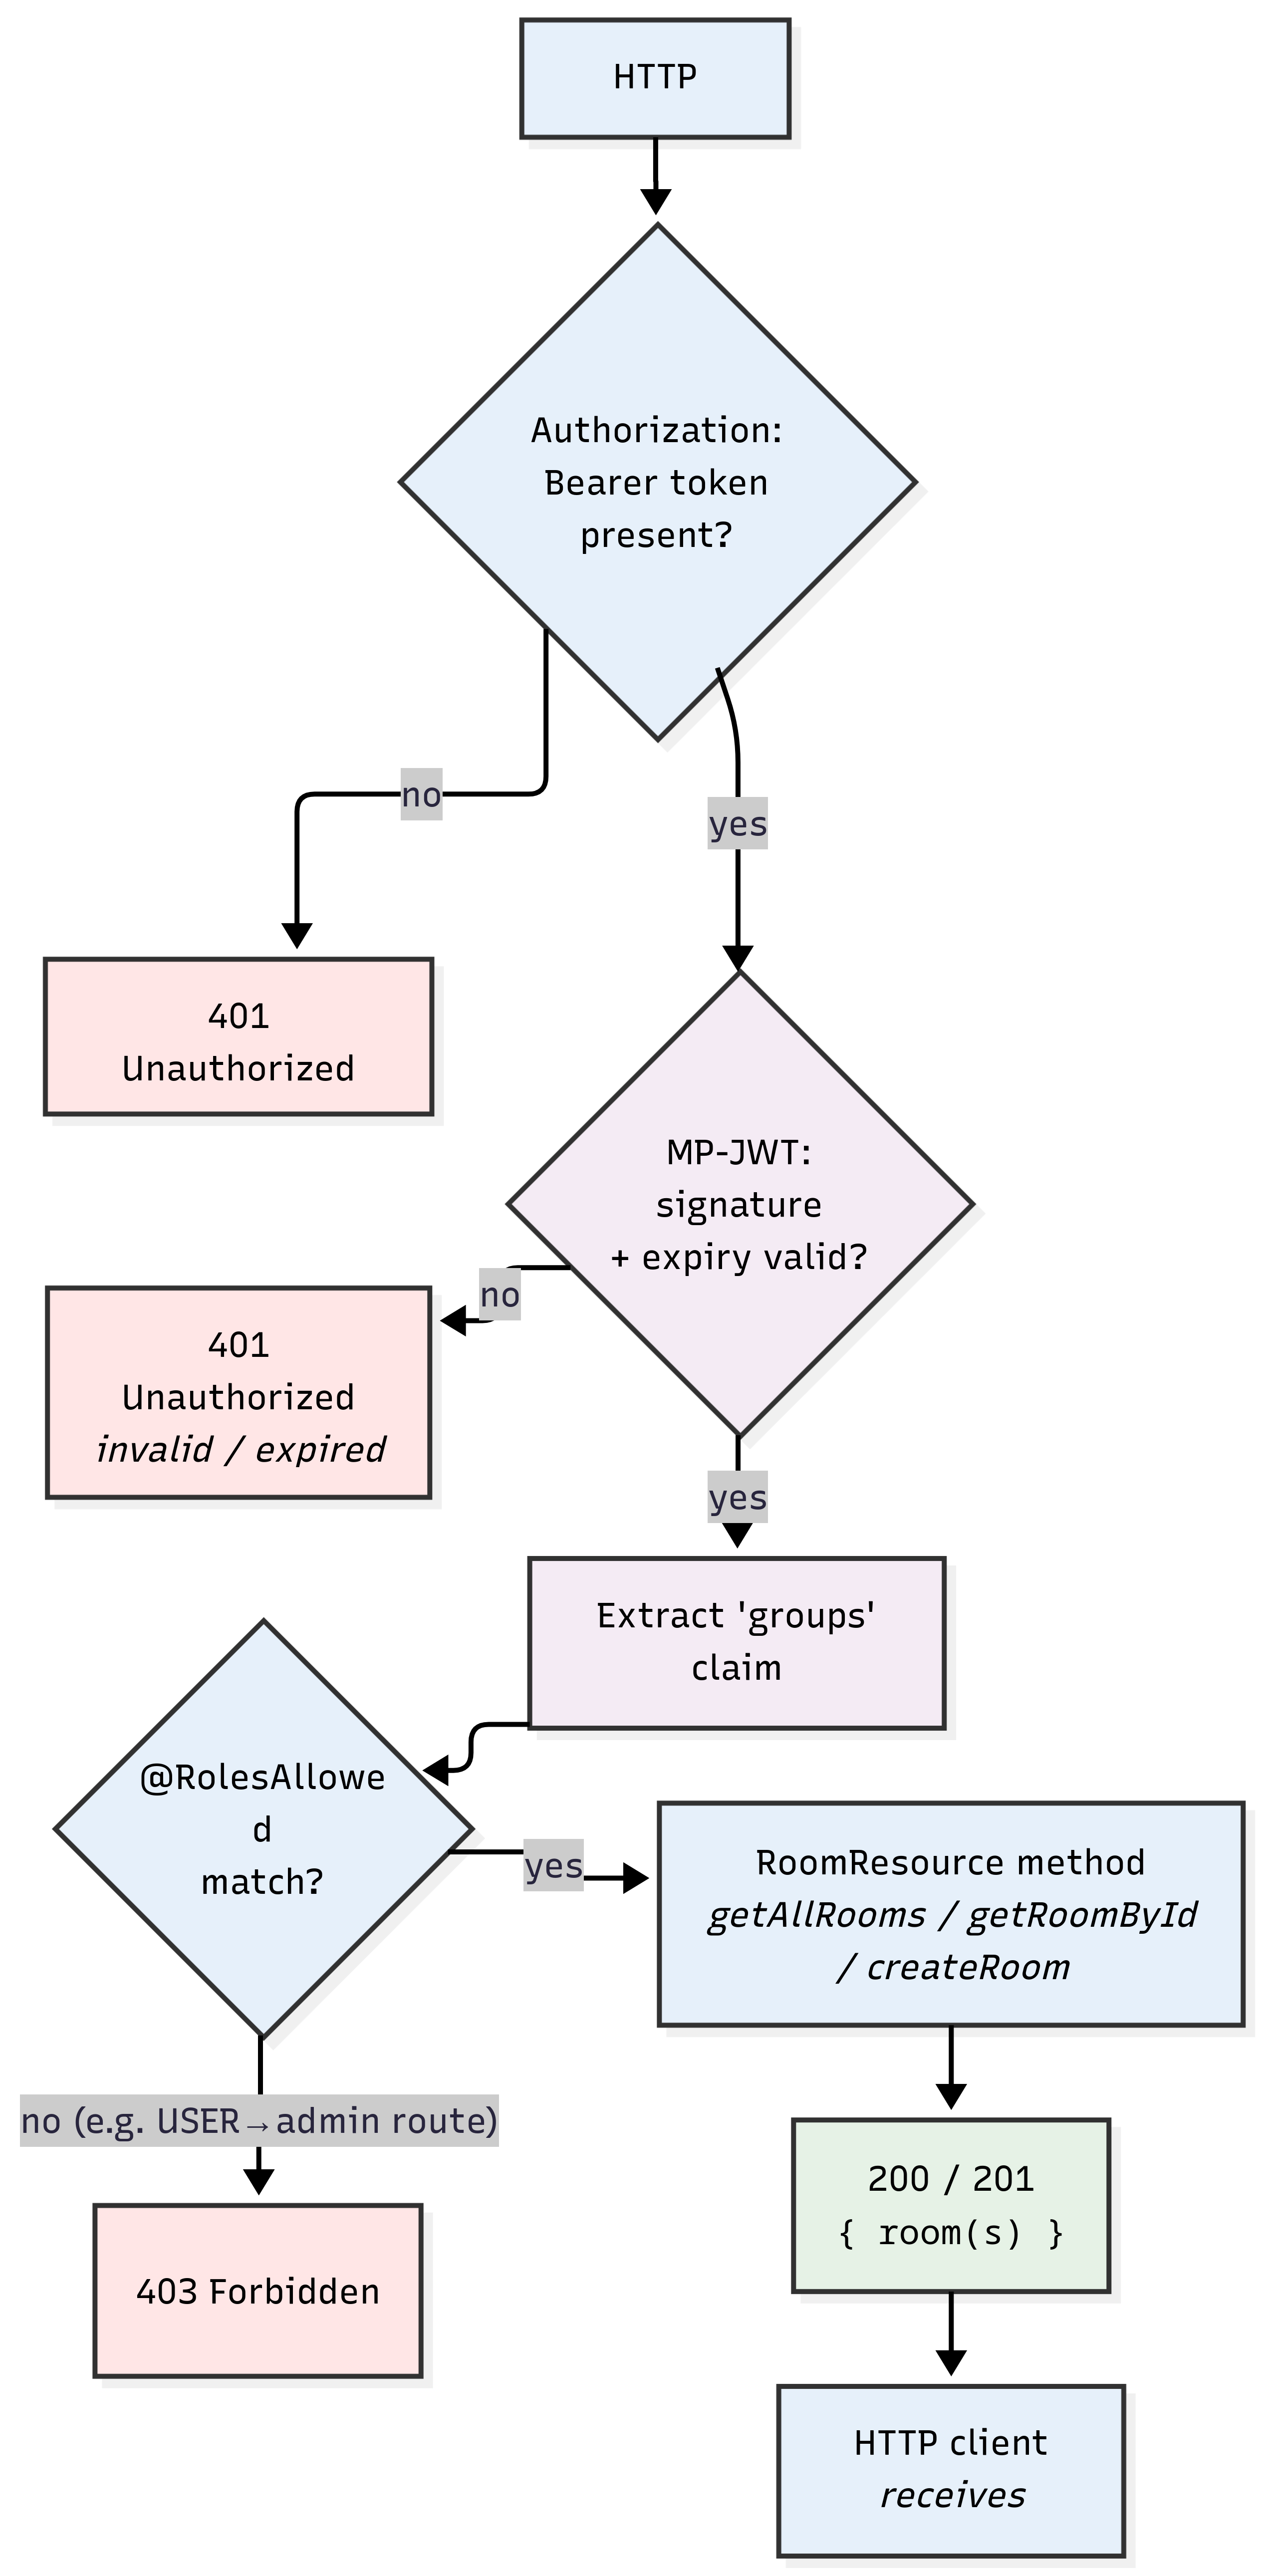
\includegraphics[width=\textwidth, height=10cm, keepaspectratio]{
		diagrams/syncspace-request-auth-flow.png
	}
	\caption{Request authorization and \ac{JWT} validation flow.}
	\label{fig:syncspace-auth}
\end{figure}

\section{Booking Logic and Data Access}
\label{app:syncspace-booking}

Data access is managed by declarative Jakarta Data interfaces (e.g.,
\texttt{UserRepository}, \texttt{RoomRepository}). A critical custom query exists
in the \texttt{BookingRepository} to guard against double-bookings, verifying
that no existing confirmed bookings for a specific room overlap with the requested
time interval.

The \texttt{BookingService} executes operations within a \texttt{@Transactional}
context. Notably, booking ownership is derived strictly from the \ac{JWT}
\texttt{sub} claim (the authenticated caller), never from client-supplied
payload IDs. The service handles both specific room requests and automatic assignments,
where the system queries for rooms matching the required capacity and type, streaming
the results to find the first available slot.

\begin{figure}[H]
	\centering
	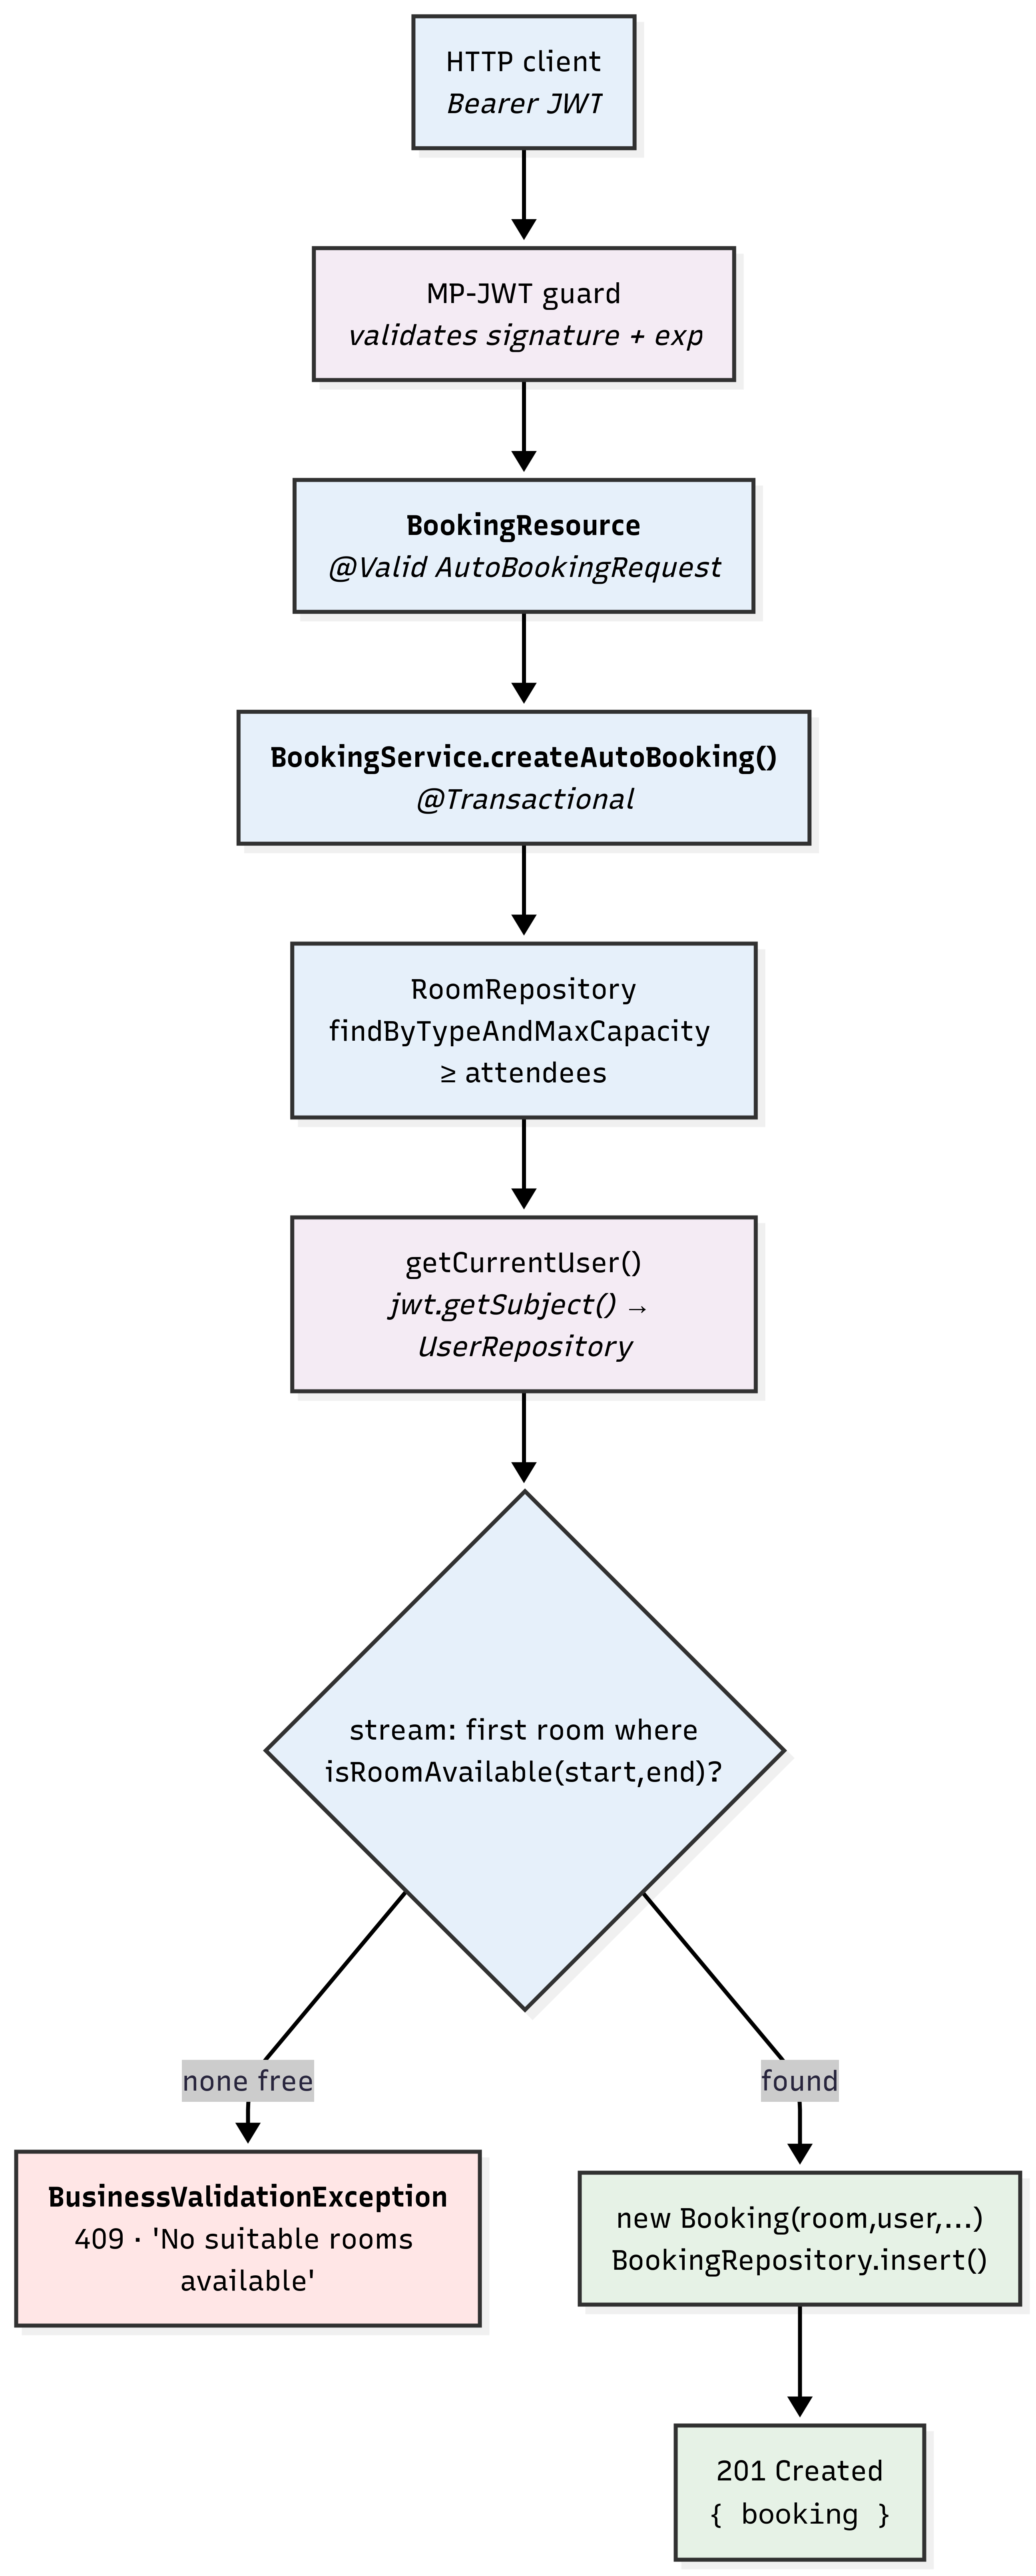
\includegraphics[width=\textwidth, height=10cm, keepaspectratio]{
		diagrams/syncspace-auto-booking-flow.png
	}
	\caption{Automatic booking assignment and validation flow.}
	\label{fig:syncspace-autobooking}
\end{figure}

\section{API Surface}
\label{app:syncspace-api}

All endpoints are prefixed with \texttt{/api/v1}. The \ac{API} exposes the
following primary operations:

\begin{table}[H]
	\centering
	\renewcommand{\arraystretch}{1.2}
	\resizebox{\linewidth}{!}{%
	\begin{tabular}{llll}
		\toprule \textbf{Method} & \textbf{Path}                  & \textbf{Auth} & \textbf{Purpose}                   \\
		\midrule \texttt{POST}   & \texttt{/auth/register}        & Public        & Create a new user                  \\
		\texttt{POST}            & \texttt{/auth/login}           & Public        & Authenticate and obtain a \ac{JWT} \\
		\texttt{POST}            & \texttt{/bookings/auto}        & \ac{JWT}      & Auto-assign a suitable room        \\
		\texttt{POST}            & \texttt{/bookings/room/\{id\}} & \ac{JWT}      & Book a specific room               \\
		\texttt{GET}             & \texttt{/rooms}                & USER/ADMIN    & List all available rooms           \\
		\texttt{POST}            & \texttt{/rooms}                & ADMIN         & Create a new room                  \\
		\bottomrule
	\end{tabular}%
	}
	\caption{Primary \ac{REST} endpoints exposed by SyncSpace.}
\end{table}

\section{Validation and Centralized Error Handling}
\label{app:syncspace-errors}

Request payloads are validated using standard Jakarta Bean Validation (\texttt{@NotNull},
\texttt{@Positive}, \texttt{@Future}). A custom class-level constraint, \texttt{@ValidDateRange},
ensures booking end times strictly follow start times, mapping violations
directly to the \texttt{endTime} property node for clearer client feedback.

To ensure clients receive consistent \ac{JSON} envelopes rather than raw
stack traces, a four-tier \ac{JAX-RS} \texttt{ExceptionMapper} hierarchy intercepts
all failures.

\begin{figure}[H]
	\centering
	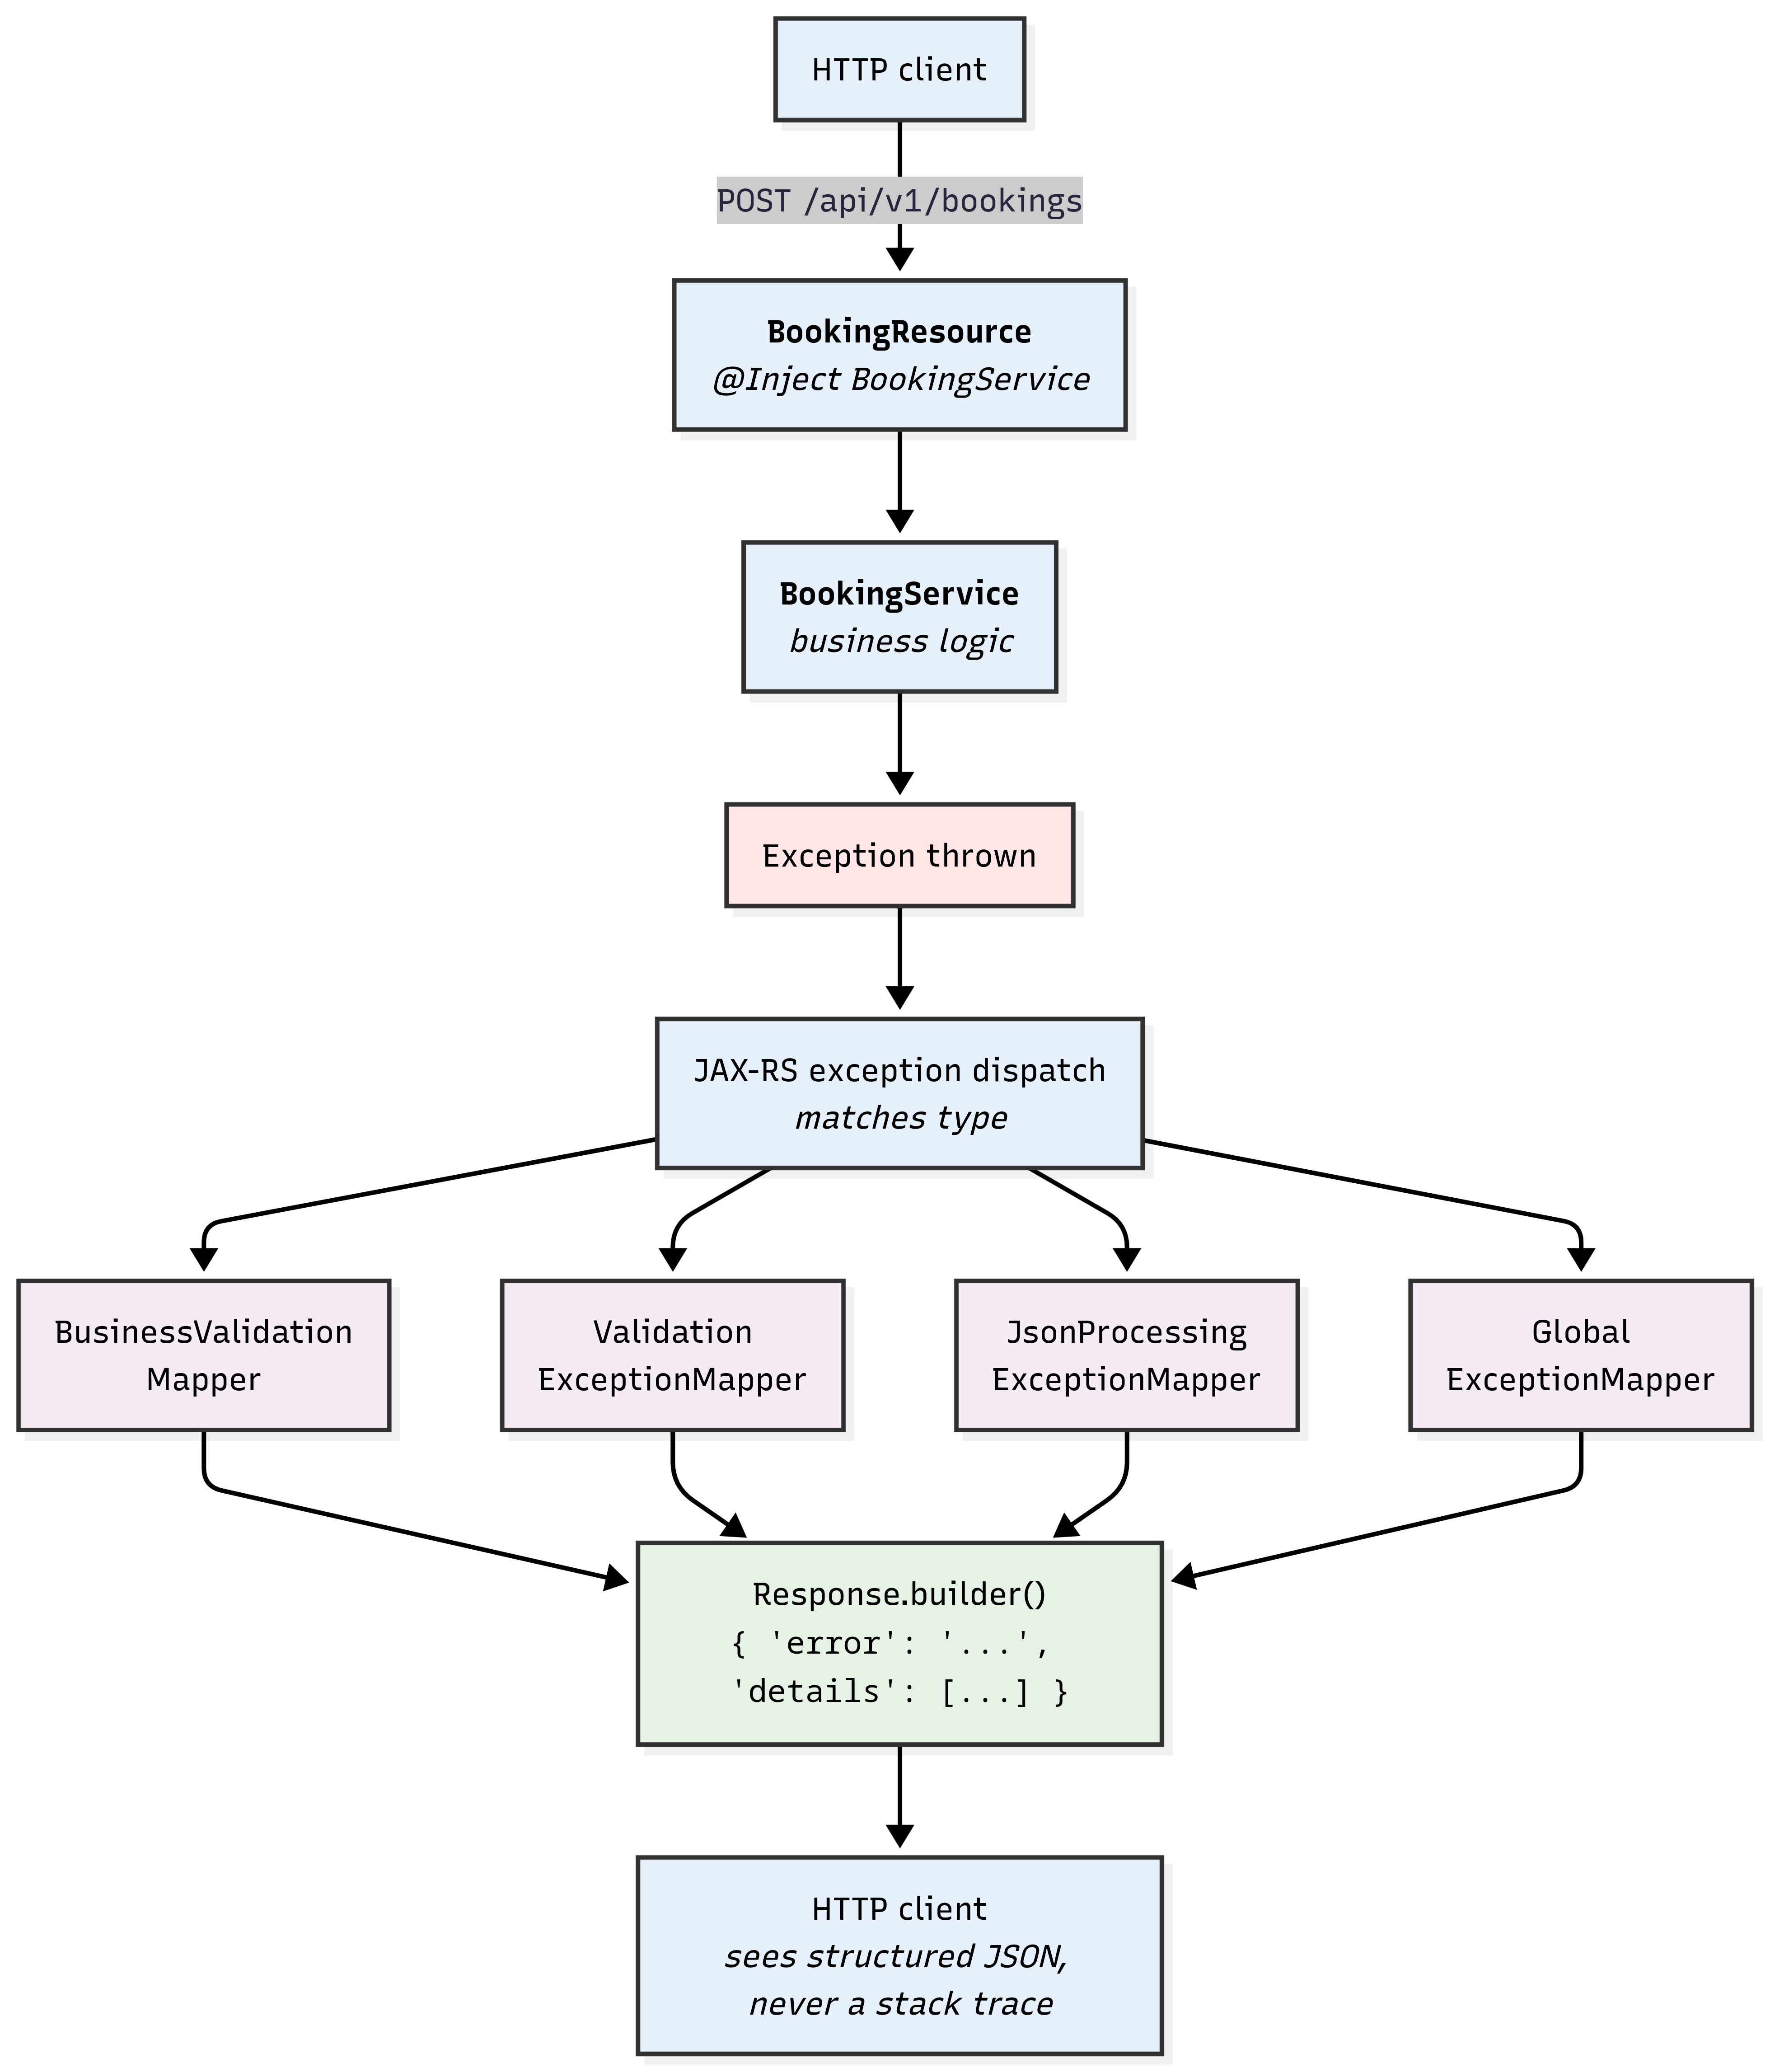
\includegraphics[width=\textwidth, height=10cm, keepaspectratio]{
		diagrams/syncspace-diagram.png
	}
	\caption{The \ac{CDI} and \ac{JAX-RS} exception-handling flow.}
	\label{fig:errormapper-appendix}
\end{figure}

The hierarchy handles specific domain exceptions (\texttt{BusinessValidationException}
for capacity or availability logic), input violations (\texttt{ConstraintViolationException}),
malformed payloads (\texttt{JsonProcessingException}), and falls back to a
\texttt{GlobalExceptionMapper} for unexpected server faults. The global
mapper securely logs the stack trace internally and returns a clean 500
response containing only a generated UUID reference.

\section{Design Highlights}
\label{app:syncspace-highlights}

The SyncSpace prototype successfully demonstrated several architectural priorities:
\begin{itemize}
	\item \textbf{Server-Derived Identity:} Utilizing \ac{JWT} claims prevents
		parameter tampering and ensures users can only book resources under their
		own identity.

	\item \textbf{Stateless Execution:} Asymmetric \ac{JWT} signatures eliminate
		the need for session state on the application server.

	\item \textbf{Declarative Persistence:} Jakarta Data drastically reduces
		boilerplate data-access code, reserving manual queries exclusively for complex
		overlap logic.

	\item \textbf{Reproducible Environments:} Integrating Datafaker with a
		CDI startup observer guarantees that developers and automated tests
		operate against a consistent, deterministic dataset on every deployment.
\end{itemize}